\subsection{Монтировки телескопов}

Монтировки телескопов разделяют на 2 основных вида (Рис.\ref{mount-equator}):
\begin{enumerate}
\item Экваториальная монтировка
\item Азимутальная монтировка
\end{enumerate}

\textit{Экваториальная монтировка}~--- монтировка, одна ось которой направлена на полюс мира (полярная ось), а другая параллельна небесному экватору (ось склонения). Крупные телескопы обычно устанавливают именно на экваториальные монтировки. Чтобы гидировать с такой монтировкой, нужно поворачивать его с постоянной скоростью вокруг полярной оси в направлении роста часового угла.

5 типов экваториальных монтировок:
\begin{enumerate}
\item Немецкая монтировка
\item Английская монтировка
\item Монтировка с рамой
\item Монтировка с ярмой
\item Американская монтировка
\end{enumerate}

\textit{Азимутальная монтировка}~--- монтировка телескопа, имеющая вертикальную и горизонтальную оси вращения, позволяющие поворачивать телескоп по высоте и азимуту. Для слежения за космическими объектами, перемещающиеся по небесной сфере вследствие суточного вращения Земли, телескоп нужно поворачивать одновременно вокруг обеих осей с разными переменными скоростями.

\begin{figure}[!h]
\centering
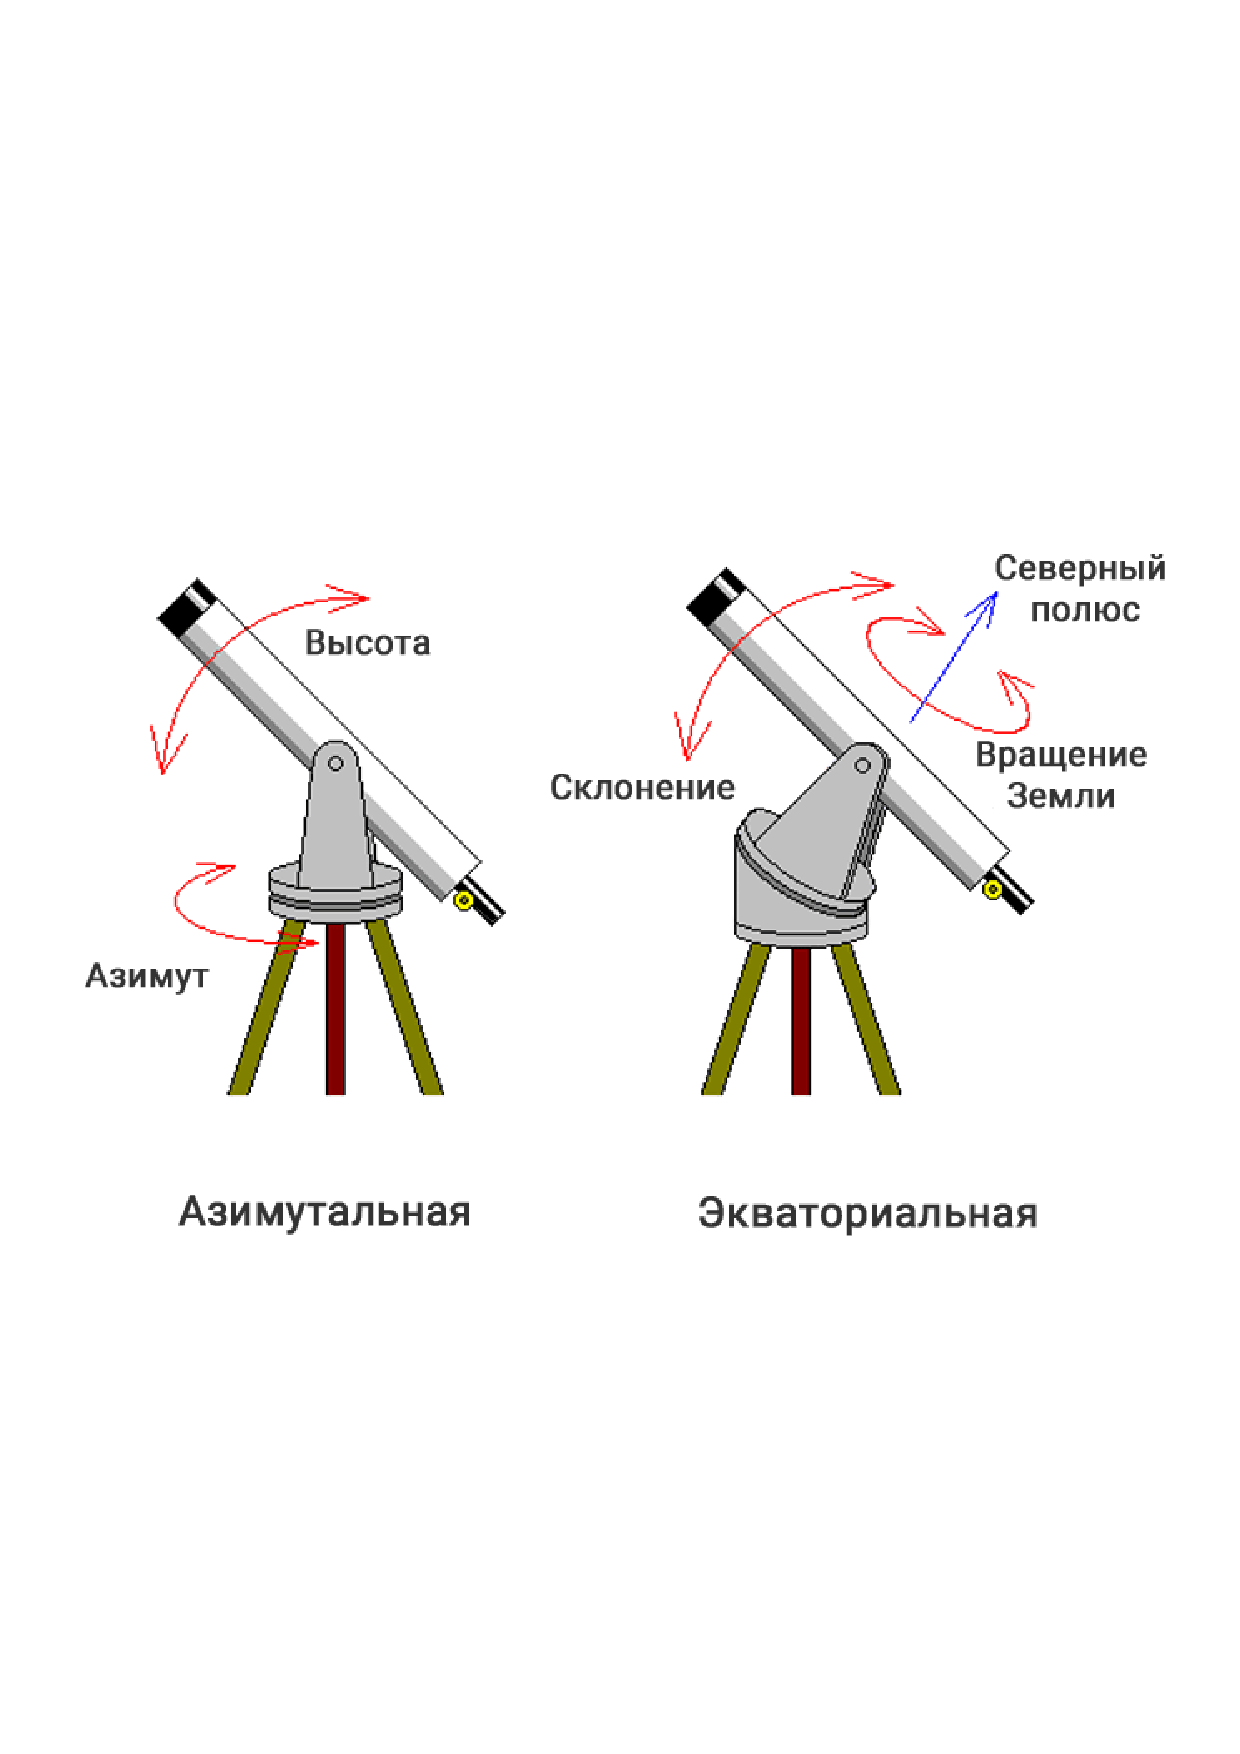
\includegraphics[width=0.85\textwidth]{mount-equator}
\caption{Виды монтировок}\label{mount-equator}
\end{figure}